%%%%%%%%%%%%%%%%%%%%%%%%%%%%%%%%%%%%%%%%%%%%%%%%%%%%%%%%%%%%%%%%%%%%%
%% This is a (brief) model paper using the achemso class
%% The document class accepts keyval options, which should include
%% the target journal and optionally the manuscript type.
%%%%%%%%%%%%%%%%%%%%%%%%%%%%%%%%%%%%%%%%%%%%%%%%%%%%%%%%%%%%%%%%%%%%%
\documentclass[journal=acscii,manuscript=article]{achemso}
% \documentclass[journal=acscii,manuscript=article,layout=twocolumn]{achemso}

%%%%%%%%%%%%%%%%%%%%%%%%%%%%%%%%%%%%%%%%%%%%%%%%%%%%%%%%%%%%%%%%%%%%%
%% Place any additional packages needed here.  Only include packages
%% which are essential, to avoid problems later.
%%%%%%%%%%%%%%%%%%%%%%%%%%%%%%%%%%%%%%%%%%%%%%%%%%%%%%%%%%%%%%%%%%%%%
\usepackage{chemformula} % Formula subscripts using \ch{}
\usepackage[T1]{fontenc} % Use modern font encodings

%%%%%%%%%%%%%%%%%%%%%%%%%%%%%%%%%%%%%%%%%%%%%%%%%%%%%%%%%%%%%%%%%%%%%
%% If issues arise when submitting your manuscript, you may want to
%% un-comment the next line.  This provides information on the
%% version of every file you have used.
%%%%%%%%%%%%%%%%%%%%%%%%%%%%%%%%%%%%%%%%%%%%%%%%%%%%%%%%%%%%%%%%%%%%%
%%\listfiles

%%%%%%%%%%%%%%%%%%%%%%%%%%%%%%%%%%%%%%%%%%%%%%%%%%%%%%%%%%%%%%%%%%%%%
%% Place any additional macros here.  Please use \newcommand* where
%% possible, and avoid layout-changing macros (which are not used
%% when typesetting).
%%%%%%%%%%%%%%%%%%%%%%%%%%%%%%%%%%%%%%%%%%%%%%%%%%%%%%%%%%%%%%%%%%%%%
\newcommand*\mycommand[1]{\texttt{\emph{#1}}}

%%%%%%%%%%%%%%%%%%%%%%%%%%%%%%%%%%%%%%%%%%%%%%%%%%%%%%%%%%%%%%%%%%%%%
%% Meta-data block
%% ---------------
%% Each author should be given as a separate \author command.
%%
%% Corresponding authors should have an e-mail given after the author
%% name as an \email command. Phone and fax numbers can be given
%% using \phone and \fax, respectively; this information is optional.
%%
%% The affiliation of authors is given after the authors; each
%% \affiliation command applies to all preceding authors not already
%% assigned an affiliation.
%%
%% The affiliation takes an option argument for the short name.  This
%% will typically be something like "University of Somewhere".
%%
%% The \altaffiliation macro should be used for new address, etc.
%% On the other hand, \alsoaffiliation is used on a per author basis
%% when authors are associated with multiple institutions.
%%%%%%%%%%%%%%%%%%%%%%%%%%%%%%%%%%%%%%%%%%%%%%%%%%%%%%%%%%%%%%%%%%%%%
\author{Daniel Vella}
\affiliation{Department of Artificial Intelligence}
\email{jean.p.ebejer@um.edu.mt} %% JP: the PI address is used, because you address will cease to exist after graduation ...
\author{Jean-Paul Ebejer}
\affiliation{Centre for Molecular Medicine and Biobanking}
% \altaffiliation{A shared footnote}
\altaffiliation{University of Malta, Msida, Malta}

%%%%%%%%%%%%%%%%%%%%%%%%%%%%%%%%%%%%%%%%%%%%%%%%%%%%%%%%%%%%%%%%%%%%%
%% The document title should be given as usual. Some journals require
%% a running title from the author: this should be supplied as an
%% optional argument to \title.
%%%%%%%%%%%%%%%%%%%%%%%%%%%%%%%%%%%%%%%%%%%%%%%%%%%%%%%%%%%%%%%%%%%%%
% \title[An \textsf{achemso} demo]
\title
  {Few-Shot Learning for Low Data Drug Discovery}

%%%%%%%%%%%%%%%%%%%%%%%%%%%%%%%%%%%%%%%%%%%%%%%%%%%%%%%%%%%%%%%%%%%%%
%% Some journals require a list of abbreviations or keywords to be
%% supplied. These should be set up here, and will be printed after
%% the title and author information, if needed.
%%%%%%%%%%%%%%%%%%%%%%%%%%%%%%%%%%%%%%%%%%%%%%%%%%%%%%%%%%%%%%%%%%%%%
\abbreviations{LBVS, Tox21, MUV, DUD-E}
\keywords{few-shot learning, machine learning, low-data, prototypical networks}  %% JP: please check

%%%%%%%%%%%%%%%%%%%%%%%%%%%%%%%%%%%%%%%%%%%%%%%%%%%%%%%%%%%%%%%%%%%%%
%% The manuscript does not need to include \maketitle, which is
%% executed automatically.
%%%%%%%%%%%%%%%%%%%%%%%%%%%%%%%%%%%%%%%%%%%%%%%%%%%%%%%%%%%%%%%%%%%%%
\begin{document}

%%%%%%%%%%%%%%%%%%%%%%%%%%%%%%%%%%%%%%%%%%%%%%%%%%%%%%%%%%%%%%%%%%%%%
%% The "tocentry" environment can be used to create an entry for the
%% graphical table of contents. It is given here as some journals
%% require that it is printed as part of the abstract page. It will
%% be automatically moved as appropriate.
%%%%%%%%%%%%%%%%%%%%%%%%%%%%%%%%%%%%%%%%%%%%%%%%%%%%%%%%%%%%%%%%%%%%%
% \begin{tocentry}

% Some journals require a graphical entry for the Table of Contents.
% This should be laid out ``print ready'' so that the sizing of the
% text is correct.

% Inside the \texttt{tocentry} environment, the font used is Helvetica
% 8\,pt, as required by \emph{Journal of the American Chemical
% Society}.

% The surrounding frame is 9\,cm by 3.5\,cm, which is the maximum
% permitted for  \emph{Journal of the American Chemical Society}
% graphical table of content entries. The box will not resize if the
% content is too big: instead it will overflow the edge of the box.

% This box and the associated title will always be printed on a
% separate page at the end of the document.

% \end{tocentry}

%%%%%%%%%%%%%%%%%%%%%%%%%%%%%%%%%%%%%%%%%%%%%%%%%%%%%%%%%%%%%%%%%%%%%
%% The abstract environment will automatically gobble the contents
%% if an abstract is not used by the target journal.
%%%%%%%%%%%%%%%%%%%%%%%%%%%%%%%%%%%%%%%%%%%%%%%%%%%%%%%%%%%%%%%%%%%%%
\begin{abstract}
  The discovery of new leads through ligand-based virtual screening in drug discovery is essentially a low-data problem, as data acquisition is both difficult and expensive to acquire. The application of conventional machine learning techniques to this problem domain is hindered by the requirement for large amounts of training data. In this work, we explore few-shot machine learning for LBVS, in which we build on the state-of-the-art, and introduce two new metric-based meta-learning techniques, Prototypical and Relation Networks, to this problem domain. We also explore the use of different embeddings and find that learned graph embeddings consistently perform better than extended-connectivity fingerprints. We conclude that the effectiveness of few-shot learning is highly dependent on the nature of the data. Few-shot learning models struggle to perform consistently on MUV and DUD-E data, in which the active compounds are structurally distinct. However, on Tox21 data, the few-shot models perform well, and we find that Prototypical Networks outperform the state of the art. Additionally, training these networks is substantially faster (up to 190\%) and therefore take a fraction of the time to train for comparable, or better, results.
\end{abstract}

%%%%%%%%%%%%%%%%%%%%%%%%%%%%%%%%%%%%%%%%%%%%%%%%%%%%%%%%%%%%%%%%%%%%%
%% Start the main part of the manuscript here.
%%%%%%%%%%%%%%%%%%%%%%%%%%%%%%%%%%%%%%%%%%%%%%%%%%%%%%%%%%%%%%%%%%%%%
\section{Introduction}

We humans exhibit a remarkable ability to learn new concepts fast and efficiently. A child seeing a cat for the first time is able to discriminate future encounters with cats from other animals. This ability is in stark contrast with conventional supervised end-to-end machine learning, which is data hungry and requires a plethora of data points to develop an effective model. Meta-learning reframes the traditional machine learning problem, allowing machine learning models to learn utilising only a few examples. Humans have an innate capability to \textit{learn how to learn}, and bridging this gap between human and machine learning is beneficial, particularly in domains where data availability or acquisition is difficult, such as the drug-discovery domain. The main goal in the drug-discovery process is the development of active compounds, that exhibit therapeutic effects against biological targets, which classifies the tested compound as a lead. The drug-discovery process comes with exorbitant costs and resource expenditure, which can exceed one billion dollars and take up to 15 years to complete \cite{hughes2011principles}. Moreover, data is also expensive and difficult to acquire, as this requires testing of numerous compounds both \textit{in-vitro} and \textit{in-vivo}. Even upon identification of leads, attrition rates are high as the compound usually fails for other reasons such as poor absorption, distribution, metabolism, excretion, or toxicology (ADMET) characteristics \cite{waring2015analysis}. It is difficult to predict such characteristics about the candidate molecule when only a small amount of related biological data is available. Therefore, the lead identification and optimisation step in drug discovery is essentially a low-data problem \cite{altae2017low}. The requirement for the plethora of training data required to train a model hinders the applicability of machine learning to lead identification and optimisation in the drug-discovery process. In the past years, the computer vision saw successful applications and advancements for low-data machine learning \cite{koch2015siamese, vinyals2016matching, snell2017prototypical, sung2018learning}. Few-shot learning relieves the burden of collecting large-scale labelled data and makes the learning of rare cases possible \cite{wang2020generalizing}. 

\begin{figure}
  \centering
  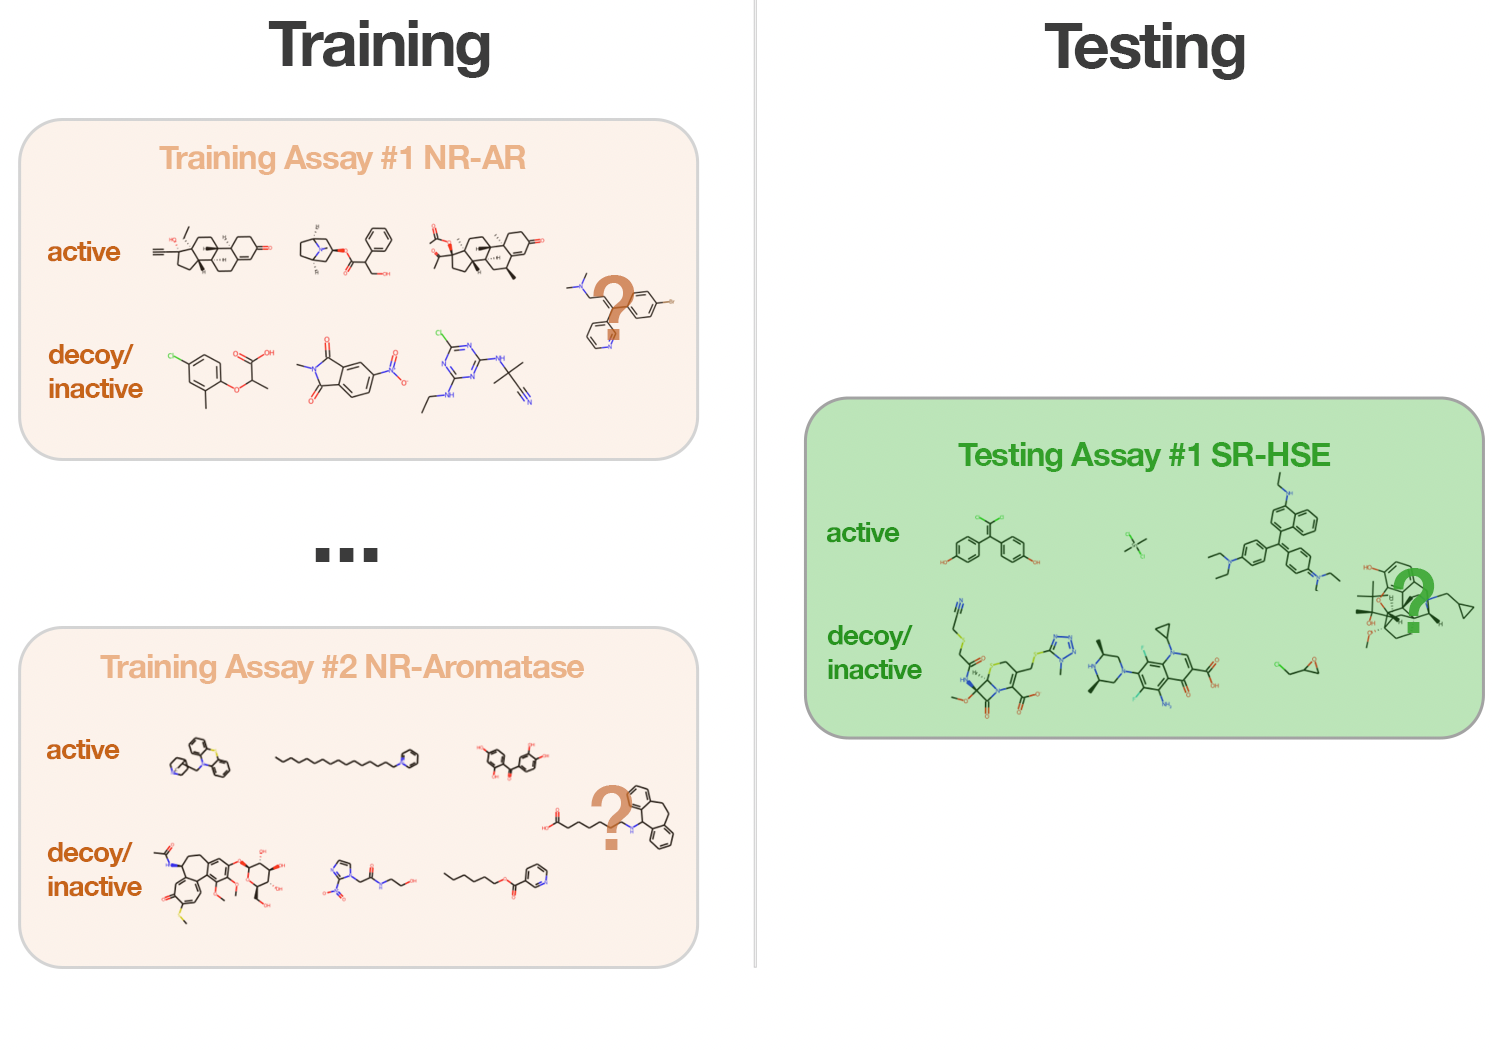
\includegraphics[width=0.8\linewidth]{img/tox21-metalearning.png}
  \caption{2-way 3-shot few-shot classification. Training a meta-learner on a set of experimental assays, and generalising for an unseen assay in the Tox-21 dataset.}
\label{fig:tox21metalearning}
\end{figure}

Building on this notion, we aim to explore few-shot learning for virtual screening to address the low-data problem in this domain. The ability for a machine learning model to learn new concepts fast with just a few training examples is invaluable for virtual screening, where data on active compounds is scarce. Meta-learning aims to achieve generalising capabilities for environments that were previously unseen during training time. In meta-learning, such as few-shot classification, we train using a variety of training tasks and optimise for performance over a distribution of tasks, including unseen ones. Learning consists of a series of episodes, each consisting of an \textit{N}-way \textit{K}-shot classification task, effectively simulating the conditions at testing time. The \textit{way} refers to the number of classes we have per task and the number of samples we have is the \textit{shot} component. These samples make up the support set \cite{snell2017prototypical}. During test time, a small support set is sampled from new, previously unseen targets, and these few data points are used by the model to generalise for the activity of query molecules against this new target \cite{vinyals2016matching}. Figure~\ref{fig:tox21metalearning} shows an example of a typical meta-learning scenario on the Tox21 dataset, where data from a set of training assays are used to train a model, which is in turn used to generalise for a new, unseen assay using a support set from this new assay. We highlight that few-shot learning in the domain under study is in contrast to other domains such as computer vision, where the trained model recognises new classes. For example, given a few images of a lion as the support set, the model must generalise for new unseen images of a lion. In this domain, the challenge is to generalise to the behaviour of molecules in experimental assays which are related but not identical to the assays in the training collection. Given a few molecules from new experimental assays, can the model predict the activity of molecules in this new assay?

\section{Related Work}

Inspired by human learning \cite{lake2015human}, few-shot learning makes use of data from similar tasks to compensate for the lack of data for the task at hand. Several successful research undertakings have exploited this paradigm \cite{koch2015siamese, vinyals2016matching, snell2017prototypical, sung2018learning}, mainly for the computer vision domain. Meta-learning refers to this ability to learn how to learn \cite{thrun2012learning, finn2017model}. Being able to learn from only a few examples is important as certain domains do not have access to the plethora of data that we see in other domains such as computer vision. This inaccessibility could be due to privacy, safety, or ethical issues. For instance, data acquisition can be problematic in the drug-discovery domain due to possible toxicity, low activity or solubility in clinical candidates. Learning with low data leads to less expensive data gathering and reduced computational cost for learning \cite{wang2020generalizing}.

\citet{altae2017low} introduce a deep-learning architecture for few-shot learning in drug discovery, building on past work in metric-based meta-learning \cite{vinyals2016matching}, in which they propose the iterative refinement long short-term memory (IterRefLSTM). IterRefLSTM builds on the Matching Networks \cite{vinyals2016matching} by introducing iterative refinement of embeddings using long-short term memory (LSTM) networks. We build on their work by applying other successful few-shot learning approaches to this problem domain. In this study, we explore the application of a number of few-shot learning architectures including, in chronological order, Siamese networks \citep{koch2015siamese}, Matching Networks \citep{vinyals2016matching}, Prototypical Networks \citep{snell2017prototypical} and Relation Networks \citep{sung2018learning}. This group of architectures fall under the umbrella of metric-based meta-learning. In our study, we embed molecule representations using graph convolution networks, and then use or learn a distance function over these embeddings. Effectively, metric-based learners seek to learn a relationship between the input embeddings in the task space. For the purposes of this study, few-shot learning refers to training with as little as one example per class, to a maximum of 10 examples per class. Training with only one example per class is referred to as one-shot learning \citep{koch2015siamese, vinyals2016matching}.

\subsection{Graph Neural Networks}

Before processing the embeddings using few-shot machine learning architectures, the SMILES molecular representations need to be represented in computational space. \citet{wu2018moleculenet} report that graph-based models outperforms conventional machine learning models on the majority of datasets, suggesting that a learned embedding is advantageous over other molecular representations. Thus, we opt for graph learned molecular representations to embed the input molecules. Graphs are natural representations of molecules, where nodes and edges represent atoms and bonds, respectively. When representing molecules, the set of vertices \textit{V} intuitively refers to atoms within a molecule, while the set of edges \textit{E} refers to the bonds that connects two atoms together (see Equation~\ref{eq_graph}). Selected properties such as atomic number, atom type, charge, and valences, among others, can be encoded in the node feature vector.

\begin{equation}\label{eq_graph}
 \mathcal{G}=(\mathcal{V}, \mathcal{E})
\end{equation}

Graph neural networks can be used to learn molecular representations by applying convolutional operators and pooling layers on the molecular graphs \cite{jiang2021could}. Embeddings learned through neural networks afford the construction of automated features, rather than fixed fingerprints. Graph neural networks are effective in transforming small molecules into real-valued vector representations, which has been found to be a productive way of processing small molecules within deep neural networks \cite{gomez2018automatic}. \citet{duvenaud2015convolutional} report that using a differentiable method reduces collisions of substructures, and the fingerprint can be optimised to contain only relevant features. The fingerprint's interpretability is enhanced as this method captures activity and similarity of substructures.

% If the graph object is our input signal, we can apply a set of operators for the function we are attempting to learn. \citet{bronstein2021geometric} propose four key building blocks for deep learning on graphs, which include linear set equivariant layers, non-linear functions, local pooling layers and set invariant layers (see Figure \ref{fig:graphlayers}). For graphs, the nodes $v$ are found on a domain $\Omega$ such that $v \in \Omega$. The nodes in $\Omega$ are stored in a feature space $C$, such that $C = \mathbb{R}^k$. Using a set of feature functions $X(\Omega, C)$, we can transform the feature space of the nodes in our domain. In the equivariant layer $B$, we can take the nodes in our domain and apply a function that transforms the features of the nodes such that $X(\Omega, C) \rightarrow X(\Omega', C')$. Equivariance allows for a function $g$ to be applied before or after this layer such that $B(g.x) = g.B(x)$. The non-linear activation functions can be applied element-wise on the features of the nodes in a graph, such that $(\sigma(x))(v) = \sigma(x(v))$. The invariant layer $Z$, which can also be referred to as a global pooling layer, in which $X(\Omega, C) \rightarrow y$, satisfies the invariant condition such that $Z(g.x) = Z(x)$ \citep{bronstein2021geometric}. 

% \begin{figure}
%   \centering
%   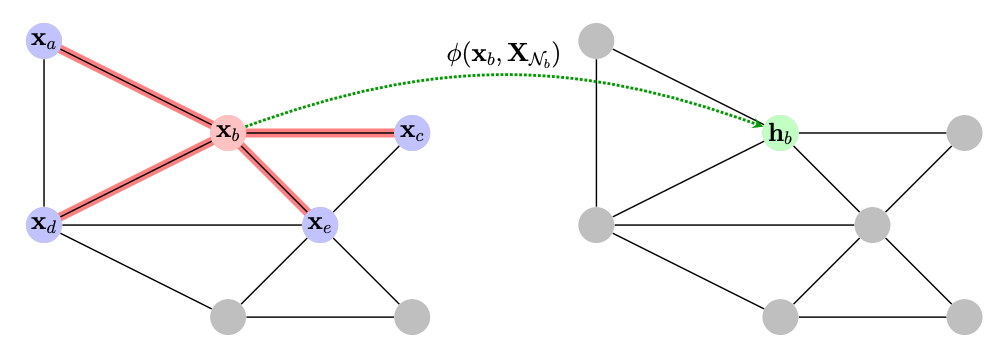
\includegraphics[width=0.9\linewidth]{img/conv-equivariance.png}
%   \caption[Graph Convolution Function]{Equivariant function in a graph, synonymous with a graph convolutional operator over neighbouring nodes. Reproduced from \citet{bronstein2021geometric}.}
%   \label{fig:convequivariance}
% \end{figure}

% In Equation~\ref{gcnequation}, the current node is included in the aggregation of neighbouring nodes through the addition of the identity matrix to the adjacency matrix to form $\hat{A}$. The diagonal node degree matrix $D$ normalises $A$, the adjacency matrix, to preserve the scale of feature vectors, such that $D^{-1}A$, which is equivalent to averaging neighbouring node features. This is further enhanced through symmetric normalisation of $A$ through $D^{-1/2}AD^{-1/2}$, which gives us the propagation rule in Equation~\ref{gcnequation} \cite{kipf2016semi}. $W$ is the weight matrix for the $l$th layer, $H$ is a neural network layer and $\sigma$ is a non-linear activation function.

% \begin{equation}
% \label{gcnequation}
% f(H^{(l)}, A) = \sigma\left( \hat{D}^{-\frac{1}{2}}\hat{A}\hat{D}^{-\frac{1}{2}}H^{(l)}W^{(l)}\right)
% \end{equation}
% where
% \begin{conditions*}
%     A & Adjacency matrix \\ 
%     $\hat{A}$ & $A + I$, in which $I$ is the identity matrix to include self-loops \\
%     $\hat{D}$ & diagonal node degree matrix of $\hat{A}$ \\
%     $\sigma(\cdot)$ & non-linear activation function \\
%     W & weight matrix for the $l$ th layer \\
%     H & neural network layer \\
%     f & non-linear function \\
% \end{conditions*}

% where
% \begin{conditions*}
%     h_j & feature size of nodes \\
%     N_i & set of neighbouring nodes i \\
%     c_ji & product of the square root of node degrees \\
%     b & learnable bias \\
%     $\sigma$ & non-linear activation function \\
% \end{conditions*}


% We then use a permutation-invariant global pooling layer, also referred to as a readout layer in literature \citep{wu2020comprehensive}. The readout layer is used to generate graph-level representations after the node features have been transformed using convolutional and local pooling layers. The readout layer is typically used at the end of the \ac{GNN} pipeline as the node representations are collapsed into a vector representing the graph \citep{wu2020comprehensive}. This vector can be further processed by multilayer perceptrons (MLP) to classify the final output, as shown in Figure \ref{fig:graphconvnetwork}.

\subsection{Metric-based few-shot learning}

The success of a few-shot learning model for metric-based meta-learning is dependent on the effectiveness of the kernel $k_\theta$, which measures the similarity between data samples (see Equation \ref{kernel}) using a metric or distance function. The models discussed in this section, excluding the benchmark model, use the support and query embeddings generated from the graph neural network to learn the kernel function.

\begin{equation}
\label{kernel}
P_\theta(y \vert \mathbf{x}, S) = \sum_{(\mathbf{x}_i, y_i) \in S} k_\theta(\mathbf{x}, \mathbf{x}_i)y_i
\end{equation}

\subsubsection{Siamese Networks}

Siamese networks \cite{bromley1993signature, koch2015siamese} are composed of two identical networks, with shared weights and parameters, taking in a pair of data samples as inputs. As the neural networks share weights, the feature extraction is maintained to the same feature space for both inputs. These identical subnetworks are finally connected in a final layer that acts as a distance function for the two outputs.

\subsubsection{Matching Networks}

Building on Siamese Networks, but instead of learning a metric function over pairs of data, the classifier learns how to define a probability distribution of output labels from query/test examples using a support set $S$ \cite{vinyals2016matching}. The classifier outputs a sum of attention weighted labels from the support set to predict the similarity between the test example and the samples from the support set. We use the same embedding function for the support and query sets to compute the molecular embeddings. Subsequently, the cosine similarity between pairs of data points between the support and query sets is computed, which is then normalised by a softmax function. The attention mechanism $a$ in $\hat{y} = \sum_{i=1}^{n} a(\hat{x}, x_i)y_i$ specifies how similar $\hat{x}$ is to each example $x$ in $S$.

\subsubsection{Prototypical Networks}

Proposed by \citet{snell2017prototypical}, these networks are similar to Matching Networks, but instead of comparing the query support to every support data point, a \textit{prototype} is calculated, which takes all the support data points per class and creates an embedding by averaging over the embeddings. The euclidean distance between the query data points and the prototypes is calculated for classification. In a one-shot learning scenario, Prototypical Networks are equivalent to Matching Networks, however, the Euclidean distance is used instead of the cosine distance used in Matching Networks.

\begin{figure}[h]
\centering
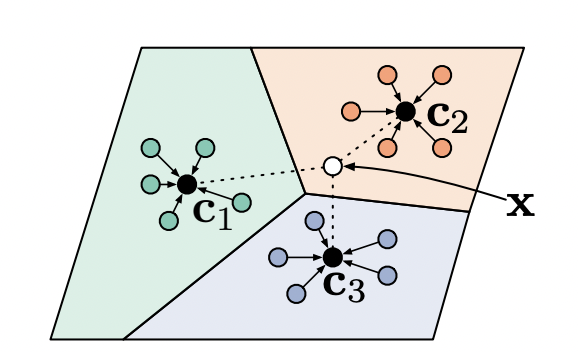
\includegraphics[width=0.7\linewidth]{img/protonets.png}
\caption{Few-shot learning in Prototypical Networks, where prototypes \textbf{$c_k$} are taken as the mean of embedded support examples for each class. Reproduced from \citet{snell2017prototypical}.}
\label{fig:protonets}
\end{figure}

\subsubsection{Relation Networks}

\citet{sung2018learning} present the Relation Network, a framework for few-shot learning, which could also be extended to zero-shot learning. The Relation Network learns a non-linear distance metric to compare support and query examples. As opposed to the aforementioned networks, this network uses a feed-forward neural network to learn a distance function in feature space. After embedding the support and query examples through an embedding function, each query example is concatenated with each of the feature maps. The resulting feature map concatenations are processed using a convolutional neural network to output a relation score vector, from which the class can be inferred.

\subsection{Iterative Refinement LSTM}

\citet{altae2017low} propose the iterative refinement long-short term memory (IterRefLSTM) to further process the resulting embeddings in a few-shot machine learning pipeline. In IterRefLSTMs two embedding functions $f(\dot|S)$ and $g(\dot|S)$ are developed simultaneously. Therefore, the embedding of the query is built iteratively with that of the support set, using information from both sets to enhance both the support and query embeddings (see Figure~\ref{fig:iterreflstm}).

\begin{figure}[h]
\centering
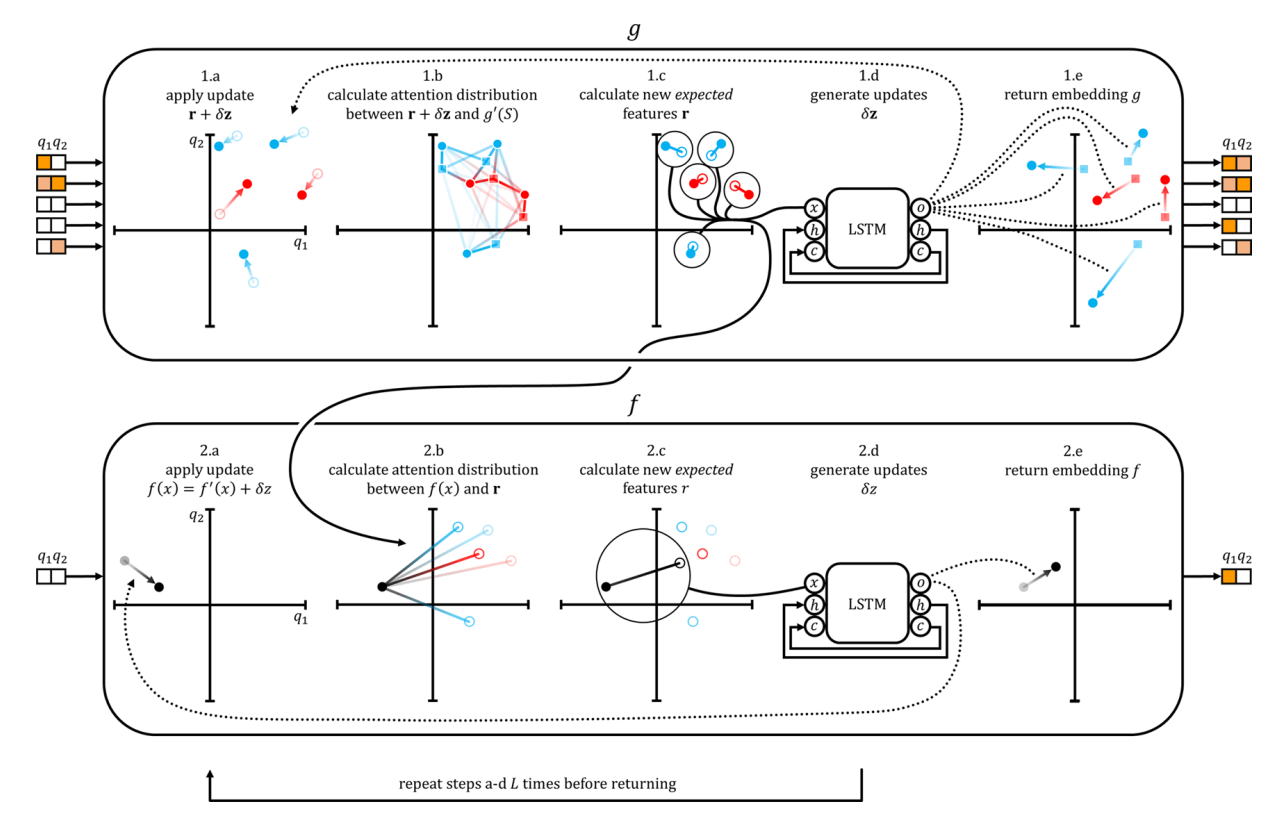
\includegraphics[width=\linewidth]{img/iterreflstm.png}
\caption{Iterative refinement of embeddings using an LSTM network. The red and blue points depict the active and inactive/decoy class, respectively. The squares depict the original embedding from $g'$. Reproduced from \citet{altae2017low}.}
\label{fig:iterreflstm}
\end{figure}

\section{Methodology}

In this work, we implement two benchmark models, and four few-shot machine learning architectures. Molecules are represented using graph objects, which are processed using graph convolutional networks (GCNs). IterRefLSTMs are used to enrich the resulting embeddings in latent space. The following sections go into the implementations in more detail.

\subsection{Datasets}

In this work, we make use of the following three datasets;

\textit{Tox21} \cite{huang2016tox21challenge}. Mainly used for lead optimisation, containing toxicity data for 12 targets \citep{tox21}. The dataset was obtained from the DeepChem AWS bucket\footnote{Accessed from: deepchemdata.s3-us-west-1.amazonaws.com/datasets/tox21.csv.gz. Last Accessed: 08/11/2021} in CSV format. The NR-AR, NR-AR-LBD, NR-AhR, NR-Aromatase, NR-ER, NR-ER-LBD, NR-PPAR-gamma, SR-ARE, SR-ATAD5 targets are reserved for training, and the remaining SR-HSE, SR-MMP, SR-p53 targets for testing.
\textit{Maximum Unbiased Validation (MUV)} \citep{rohrer2009maximum}. Based on PubChem BioAssays, used for validating virtual screening techniques against 17 different targets \citep{rohrer2009maximum}. The dataset was obtained from the DeepChem AWS bucket\footnote{Accessed from: deepchemdata.s3-us-west-1.amazonaws.com/datasets/muv.csv.gz. Last Accessed: 08/11/2021} in CSV format. A total of 12 targets (MUV-466 - MUV-810) are reserved for training, while MUV-832, MUV-846, MUV-852, MUV-858, and MUV-859 are reserved for testing.
\textit{Directory of Useful Decoys (Enhanced) (DUD-E)} \cite{mysinger2012directory}. Used for benchmarking virtual screening techniques by introducing a number of active compounds against specific targets. For each active, a number of \textit{decoys} with similar physical properties, but different topologies, are made available. For this research study, we made use of the GPCR subset of the DUD-E dataset \citep{mysinger2012directory}. The data was obtained directly from the DUD-E website.\footnote{Accessed from: http://dude.docking.org/subsets. Last Accessed: 08/11/2021} The AA2AR, DRD3, and ADRB1 are used for training. Two targets are reserved for testing, in which ADRB2 contains decoys that are auto-generated against a set of known active ligands, while for the CXCR4 target these are hand-picked. 

\begin{table}[h]
\centering
\caption{Number of actives and inactives/decoys across all targets in the datasets used. Figures in parentheses show the percentage of the total compounds in the dataset.}
\begin{tabular}{@{}crr@{}}
\hline
Dataset & Actives & Inactives/Decoys \\
\hline
Tox21 & 4,149 (7.04\%) & 54,746 (92.96\%) \\
\hline
MUV & 347 (0.20\%) & 175,990 (99.80\%) \\
\hline
DUD-E (GPCR) & 1,249 (1.45\%) & 84,856 (98.55\%) \\
\end{tabular}
\label{table:datasetimbalance}
\end{table}

\subsection{Molecular Representations}

We first create a molecular graph from the SMILES string using RDKit, an open-source toolkit for cheminformatics. Standardisation of compounds according to a set of well-defined and consistent rules and conventions is of utmost importance to maintain uniformity and integrity across the data being used. \citet{bento2020open} present an open source chemical structure curation pipeline based on RDKit for validating and standardising chemical structures, which follow FDA/IUPAC guidelines \citep{brecher2006graphical, food2007substance}. Their work is available in the ChEMBL Structure Pipeline package \cite{bento2020open} and is used to standardise the molecules in our pipeline. We then create one-hot encoded features for the atoms in each molecule, namely, atom type, atomic number, atom degree, explicit valence, hybridisation, formal charge, number of radical electrons, and aromaticity. Self loops are added to every node in the generated graph, so aggregation functions during message passing consider the features of the node itself. The order of the atoms follows the canonical order of the atoms assigned through RDKit. We make use of the DGL LifeSci \cite{dgllife} library to create the graph objects and subsequently process them using the DGL library \cite{wang2019dgl}.


\subsection{Machine Learning Models}

Before processing the molecular graph, we first learn an embedding using graph neural networks. Four different architectures, including Siamese, Matching, Prototypical and Relation Networks, process the learned graph embeddings to train our meta-learner. IterRefLSTMs are utilised to refine the latent space embeddings.
\begin{figure}[h]
  \centering
  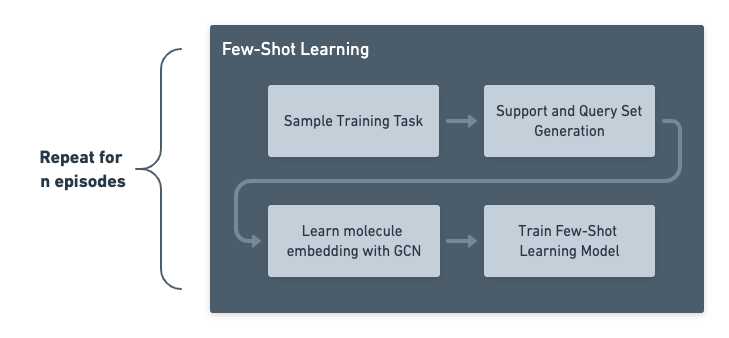
\includegraphics[width=0.9\linewidth]{img/episodic-learning.png}
  \caption{Episodic learning schematic}
  \label{fig:episodiclearning}
\end{figure}

\begin{figure*}
  \centering
  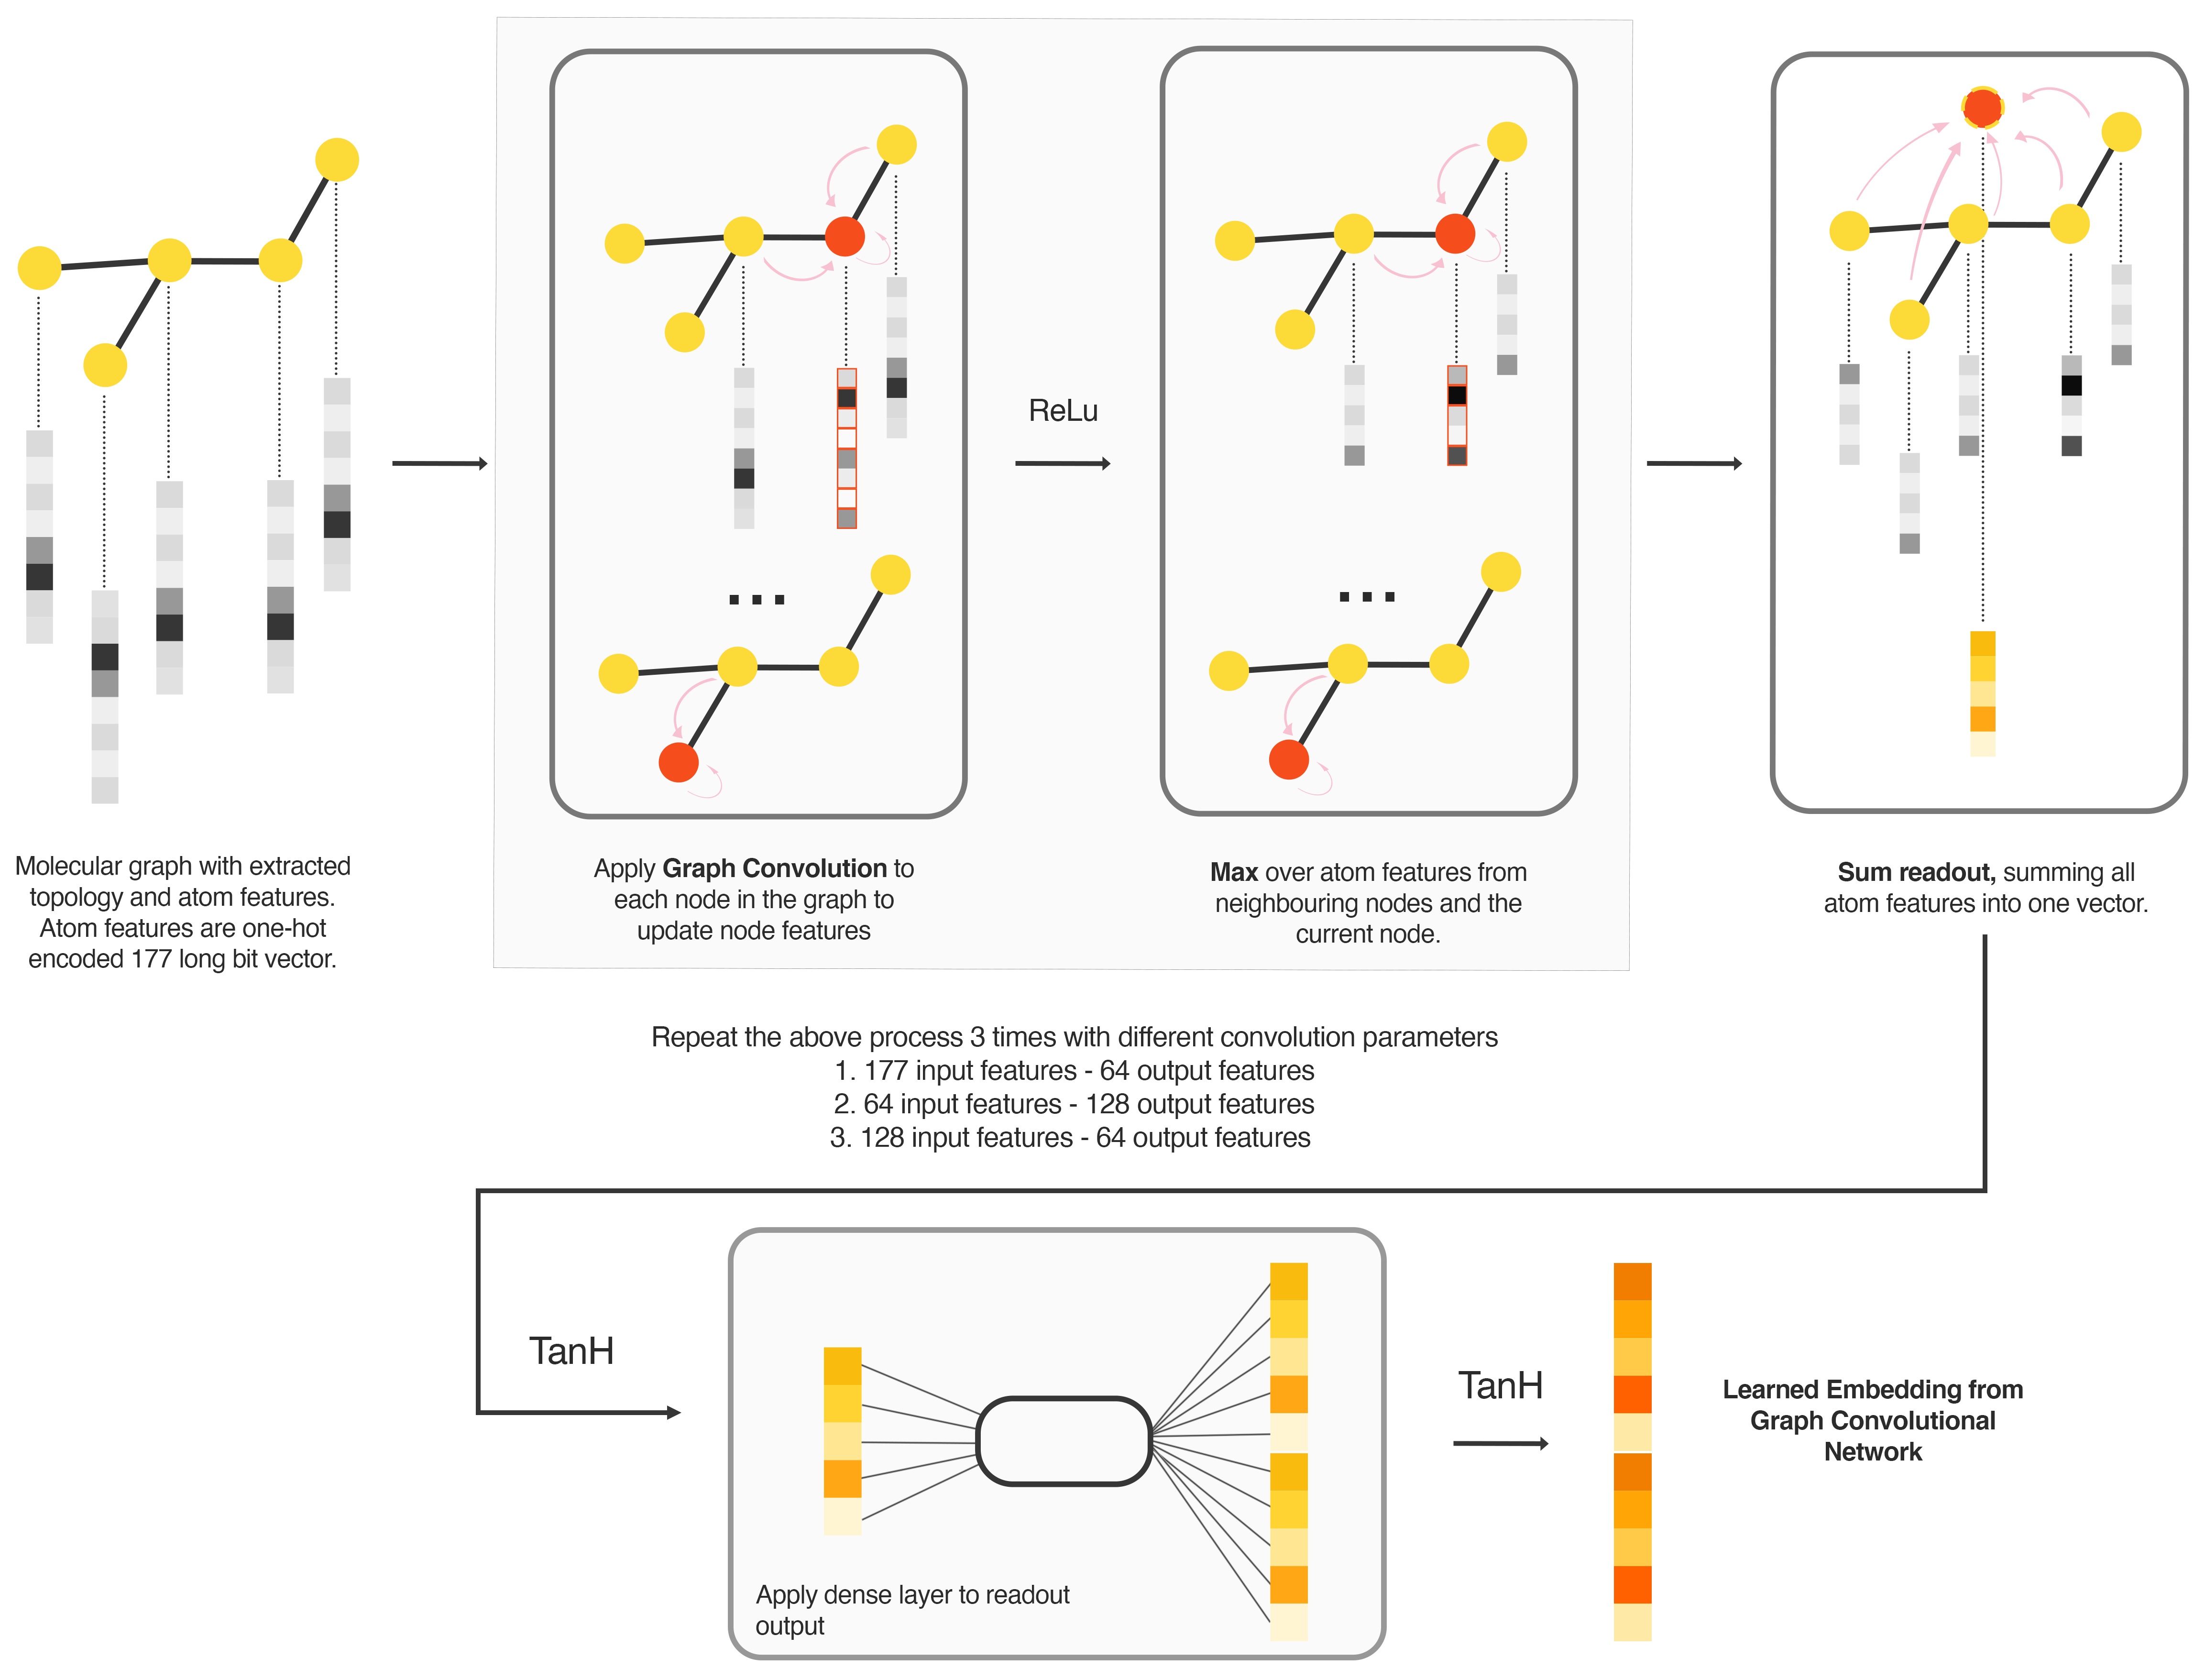
\includegraphics[width=0.75\textwidth]{img/DVGCNArchi.png}
  \caption{Learning an embedding through a Graph Convolutional Network (GCN). The molecule, represented as a graph object with nodes, edges, and atom features, is processed using graph convolutions. A max message-passing function over the current and neighbouring nodes follows each convolution layer. After this process, a sum readout aggregates all atom features into one vector. A TanH function activates this vector, and a dense linear layer processes the output vector. A non-linear TanH function activates this vector to yield the final learned molecular embedding.}
  \label{fig:dvgcnarchi}
\end{figure*}

\subsubsection{Graph Convolutional Networks}

Graph convolutional networks (GCNs) are used to learn embeddings for the support and query molecules in latent space. Figure~\ref{fig:dvgcnarchi} illustrates the GCN pipeline to learn a molecular embedding. In our study, we make use of the convolutional operator from \citet{kipf2016semi} to process graphs and learn the molecular embeddings. The convolutional layer can be mathematically defined through Equation~\ref{gcnequation2}. $h_j$ is the feature set of the node, $N_i$ is the set of neighbouring nodes $i$, $b$ is the learnable bias, and $c_ji$ is the product of the square root of node degrees. From a message-passing perspective, this can be summarised into the following steps for every node feature space $u$;

\begin{equation}
\label{gcnequation2}
h_i^{(l+1)} = \sigma(b^{(l)} + \sum_{j\in\mathcal{N}(i)}\frac{1}{c_{ji}}h_j^{(l)}W^{(l)})
\end{equation}

\begin{enumerate}
    \item Aggregating the neighbouring representations $h_v$, producing an intermediate representation $\hat{h}_u$.
    \item Transforming $\hat{h}_u$ through a linear projection and a non-linearity function such that $h_u = f(W_u \hat{h}_u)$ \citep{kipf2016semi}.
\end{enumerate}

Three convolutional layers are present in our architecture, after which a maximum function aggregating the node features with the maximum value of the neighbours and the node itself is applied. We highlight that this is not a coarsening operation, as the number of nodes remain the same. Finally, we apply a global pooling layer (readout), in which we sum over the node features of the graph (see Equation~\ref{gcnequationsum}). A linear transformation is applied to the output from the read-out layer, followed by a non-linear activation function, for which we use a hyperbolic tangent function (TanH), outputting the final molecule embedding.

\begin{equation}
\label{gcnequationsum}
r^{(i)} = \sum_{k=1}^{N_i} x^{(i)}_k
\end{equation}


\subsubsection{Benchmark}

We make use of a Random Forest model with 100 decision trees and a Graph Convolutional Network (GCN) to build a baseline to benchmark the purpose-built few-shot learning models. For the random forest model, ECFP representations of the molecules of size 2048 bits are used for the classification task. Meanwhile, the same GCN architecture used for the few-shot learning models is used for the benchmark. The only addition to the architecture is a final linear layer that takes as input 128 features, which is the size of the embedding used for the experiments to follow, and outputs a feature of size one, onto which we apply a non-linear function, in this case a Sigmoid function, to output the probabilities for a Boolean target (${0, 1}$). These two models are trained on a small support set, sampled from the targets assigned for testing. The remaining data for the designated target is used for testing.

\subsubsection{Few-Shot Learning Models}

Episodic learning is used to train a few-shot machine learning model. \citet{vinyals2016matching} suggest that conditions during training must match those during testing. Training consists of a sequence of learning problems where the model is supplied with a \textit{support} set and a corresponding \textit{query} set. The support set consists of a few molecules sampled from each class, in our case representing the active molecules and the inactives/decoys. We consider \textit{N-way K-shot} classification tasks, where the support set contains \textit{N} classes and \textit{K} labelled molecules. \textit{N} is always assigned a value of two as we are attempting to solve a binary classification problem, whereby the model tries to classify the query molecules as active or inactive in a specific experimental assay. We experimented with a varying number of molecules for the support sets, however the minimum limit was set to one compound per class, while the maximum was set to 10 compounds per class. The \textit{2-way N-shot} formulation is what the model is presented with at test time. We sample a total of 128 query molecules for each episode, which is composed of a balanced combination of molecules from each class. If the active class for a specific target contains less than 64 molecules, the active molecules are over-sampled such that each query set contains 64 actives. We reproduce the work of \citet{altae2017low} from scratch and also apply the IterRefLSTM to the embeddings from all other networks to effectively compare our contribution to past work. Additionally, we also provide implementations for the Prototypical Networks and Relation Networks. All the experiments are run on Google Colaboratory and all implementations are open-sourced on GitHub.\footnote{Accessed From: https://github.com/danielvlla/Few-Shot-Learning-for-Low-Data-Drug-Discovery}

% \makebox[0pt][l]{%
% \begin{minipage}{\linewidth}
% \centering
%     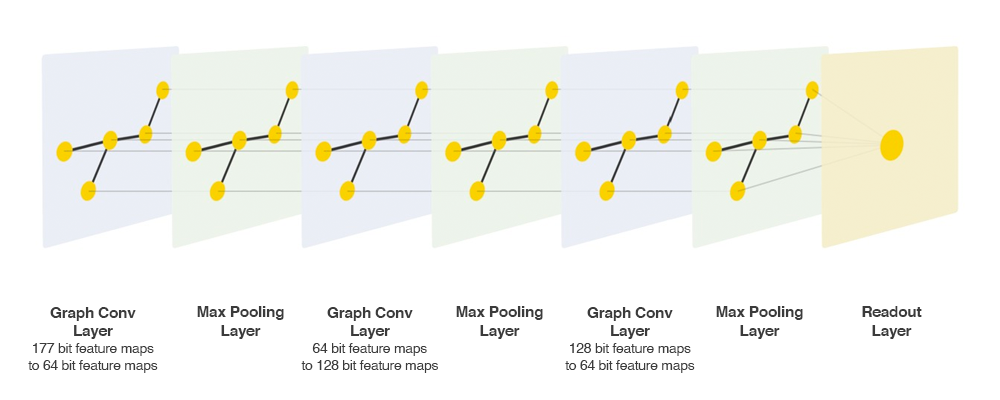
\includegraphics[width=1\linewidth]{img/gcn-layers.png}
%   \captionof{figure}{Graph processing layers in our GCN implementation. The graph convolution layers apply operations on each individual node's feature maps based on neighbouring nodes. A ReLU function activates the output from each convolutional layer. A TanH function activates the final readout layer.}
%  \label{fig:dvgcnarchi2}
% \end{minipage}
% }

\section{Results}

Performance evaluation is carried out using Receiver Operator Characteristic AUC (ROC-AUC) and Precision-Recall Area Under the Curve (PR-AUC) metrics. The state-of-the-art \cite{altae2017low} only reports ROC results, however, this metric alone does not fully encompass the nature of the performance of the machine learning models due to the hihgly imbalanced nature of the data at hand. In virtual screening, the detection of rare events (equivalent to our minority active class) holds significant importance, as active compounds against a specific target should be identified from the compound database. However, we do not disregard the importance of correct classification of the majority inactive/decoy class, as this is also important for filtering out thousands of screened compounds. As the active class is the minority class, PRC are used to evaluate how well the model can classify the active class. A high area under the PRC indicates high recall and high precision. The former is related to a low false negative rate, meaning active compounds incorrectly classified as inactive/decoys, while high precision is attributed by a low false positive rate, meaning compounds classified as active when in fact they are inactive/decoys. The ideal scenario for predicting the minority active class is thus one where we achieve high recall and high precision. As our data contains a lot of negative examples, there is a higher chance of these being predicted as false positives. On the other hand, we have much fewer active examples which could be predicted as false negatives. Given that the active class is in such a minority, even a small false positive rate could result in high numbers of false positives, due to the high number of the negative class examples. In this scenario, the precision will be low as we are predicting a lot of false positives when compared to true positives. We can also have a scenario of high recall with low precision. In this scenario, we have a high number of incorrect predictions as the model returns a lot of false positives, but it correctly predicts most of the active class as it has high recall. On the other hand, if we achieve high precision with low recall, most of the predictions are correct as we have a high number of true positives when compared to false positives.

The notation K+/K- used in the tables to follow signify the composition of the support set consisting of a number of actives and inactives/decoys respectively. Each model is evaluated 20 times per target, with a randomly sampled support set for each round. The tabulated results are the mean values from these 20 rounds, encompassing all the test targets, along with the standard deviation for each mean.

\subsection{Tox21}

When testing the machine learning models on the Tox21 dataset, the few-shot learning models outperform the baseline models. This performance is in line with that reported by \citet{altae2017low}. In line with the established state-of-the-art, the MN with IterRefLSTM performs well and obtain the best ROC results in a number of experiments. The fact that the same implementation for the Matching Networks (MNs) obtained slightly better results (1-14\% across the five support set experiments) than the state-of-the-art work, can be attributed to the set of atom descriptors used for the initial graph representations. Our few-shot learning architecture implementation is identical to their work, but different hyperparameters in the implementation which were not clear in the original work could also contribute to variations in results. Hence, we focus mainly on the performance of how our implementations performed against each other. The results from the Prototypical Networks (PNs) overall outperform the results from the MNs. Meanwhile, MNs and PNs, overall outperform Relation Networks (RNs) in both ROC and PRC performance. Results for one shot-learning do not provide a clear-cut choice between our implementations for MNs and PNs with the IterRefLSTM. They both achieve comparable performance on Tox21 targets for one-shot learning. The performance of MNs for this scenario is consistent with the state-of-the-art work. Based on the underlying theories of both architectures, the results are consistent with our expectations. In a one-shot learning scenario, MNs and PNs are conceptually similar. The \textit{prototypes} in PNs are a mean of all embeddings for each class in the support set. The euclidean distance between the \textit{prototypes} and each embedding from the query set is calculated to predict the query's activity. As in one-shot learning we only have one example per class, the \textit{prototypes} are equivalent to the embedding for each class, making this identical to MNs. The difference lies in the distance function used as for MNs we use the cosine distance, while for PNs, we make use of the euclidean distance, as proposed in the original literature which introduced these two techniques.

\begin{table*}
\caption{Mean ROC-AUC and PRC-AUC Scores with standard deviation for ML Models for the Tox21 Test Targets over 20 rounds of testing. Bold text illustrates the best obtained value. The first column shows the composition of the support set.}
\centering
% \ra{1.3}
% {\renewcommand{\arraystretch}{1}}
\resizebox{\textwidth}{!}{%
\begin{tabular}{@{}cccccccc@{}}
\hline
\textbf{Tox21} & \textbf{Metric} & \textbf{RF} & \textbf{Graph Conv} & \textbf{SiameseNet} & \textbf{MatchingNet} & \textbf{ProtoNet} & \textbf{RelationNet} \\
\hline
10+/10- & ROC & 0.617 ± 0.060 & 0.620 ± 0.065 & 0.825 ± 0.043 & 0.824 ± 0.022 & \textbf{0.826 ± 0.034} & 0.814 ± 0.030 \\ & PRC & 0.158 ± 0.102 & 0.150 ± 0.095 & 0.226 ± 0.107 & 0.367 ± 0.105 & \textbf{0.384 ± 0.105} & 0.360 ± 0.102\\
\hline
5+/10- & ROC & 0.602 ± 0.059 & 0.610 ± 0.062 & 0.828 ± 0.069 & \textbf{0.824 ± 0.033} & 0.823 ± 0.038 & 0.822 ± 0.023 \\ & PRC & 0.148 ± 0.090 & 0.152 ± 0.094 & 0.190 ± 0.094 & 0.369 ± 0.110 & \textbf{0.388 ± 0.111} & 0.355 ± 0.104\\
\hline
1+/10- & ROC & 0.563 ± 0.068 & 0.558 ± 0.076 & 0.836 ± 0.138 & 0.822 ± 0.025 & \textbf{0.826 ± 0.032} & 0.814 ± 0.028 \\ & PRC & 0.128 ± 0.084 & 0.126 ± 0.075 & 0.099 ± 0.093 & 0.301 ± 0.103 & \textbf{0.384 ± 0.096} & 0.325 ± 0.103\\
\hline
1+/5- & ROC & 0.534 ± 0.066 & 0.559 ± 0.090 & 0.807 ± 0.159 & \textbf{0.820 ± 0.033} & \textbf{0.820 ± 0.033} & 0.819 ± 0.023 \\ & PRC & 0.112 ± 0.059 & 0.128 ± 0.080 & 0.106 ± 0.086 & 0.339 ± 0.115 & \textbf{0.362 ± 0.106} & 0.318 ± 0.108\\
\hline
1+/1- & ROC & 0.550 ± 0.061 & 0.548 ± 0.102 & 0.818 ± 0.075 & 0.819 ± 0.036 & \textbf{0.820 ± 0.030} & 0.813 ± 0.029 \\ & PRC & 0.118 ± 0.068 & 0.123 ± 0.082 & 0.198 ± 0.102 & 0.352 ± 0.121 & \textbf{0.373 ± 0.102} & 0.342 ± 0.093\\
\hline
\end{tabular}
}
\label{table:Tox21-mean}
\end{table*}

\subsection{MUV}

Each active in the MUV dataset is structurally distinct from the other, making each data sample maximally informative. Therefore, structural similarities cannot be exploited on unseen active molecules. The baseline benchmark tests consistently outperformed few-shot learning techniques. \citet{altae2017low} report that the results obtained through the GCNs baseline also struggle in performance, however, from our tests and statistical analysis we find that this is not the case for all MUV targets. For most targets, there is no significant difference between the scores obtained through the RFs and GCNs baselines. RNs obtain the best ROC scores in one instance on the MUV-832 target when trained with a 1+/10- support set, obtaining a mean ROC-AUC score of $0.683 \pm 0.010$. However, this result is not consistent and the performance is only observed in this single instance. Other than this single instance, our results are consistent with the conclusion from the state-of-the-art that baseline machine learning outperforms few-shot machine learning techniques on the MUV dataset.

\begin{table*}
\caption{Mean ROC-AUC and PRC-AUC Scores with standard deviation for ML Models for MUV Test Targets over 20 rounds of testing. Bold text illustrates the best obtained value. The first column shows the composition of the support set.}
\centering
\resizebox{\textwidth}{!}{%
\begin{tabular}{@{}cccccccc@{}}
\hline
\textbf{MUV} & \textbf{Metric} & \textbf{RF} & \textbf{Graph Conv} & \textbf{SiameseNet} & \textbf{MatchingNet} & \textbf{ProtoNet} & \textbf{RelationNet} \\
\hline
10+/10- & ROC & \textbf{0.728 ± 0.145} & 0.713 ± 0.133 & 0.562 ± 0.046 & 0.628 ± 0.096 & 0.599 ± 0.085 & 0.490 ± 0.071 \\ & PRC & \textbf{0.066 ± 0.073} & 0.009 ± 0.012 & 0.001 ± 0.000 & 0.007 ± 0.010 & 0.003 ± 0.002 & 0.002 ± 0.001\\
\hline
5+/10- & ROC & \textbf{0.696 ± 0.132} & 0.666 ± 0.115 & 0.550 ± 0.054 & 0.516 ± 0.085 & 0.576 ± 0.055 & 0.502 ± 0.072 \\ & PRC & \textbf{0.071 ± 0.076} & 0.015 ± 0.022 & 0.001 ± 0.001 & 0.003 ± 0.002 & 0.003 ± 0.002 & 0.003 ± 0.002\\
\hline
1+/10- & ROC & \textbf{0.599 ± 0.104} & 0.585 ± 0.116 & 0.648 ± 0.158 & 0.492 ± 0.082 & 0.540 ± 0.053 & 0.547 ± 0.090 \\ & PRC & \textbf{0.021 ± 0.032} & 0.006 ± 0.008 & 0.001 ± 0.002 & 0.002 ± 0.001 & 0.003 ± 0.002 & 0.003 ± 0.002\\
\hline
1+/5- & ROC & \textbf{0.587 ± 0.106} & 0.585 ± 0.126 & 0.613 ± 0.179 & 0.461 ± 0.046 & 0.494 ± 0.050 & 0.500 ± 0.000 \\ & PRC & \textbf{0.027 ± 0.040} & 0.006 ± 0.008 & 0.001 ± 0.002 & 0.002 ± 0.001 & 0.002 ± 0.001 & 0.002 ± 0.000\\
\hline
1+/1- & ROC & 0.573 ± 0.103 & \textbf{0.577 ± 0.147} & 0.620 ± 0.138 & 0.507 ± 0.037 & 0.505 ± 0.030 & 0.484 ± 0.060 \\ & PRC & \textbf{0.022 ± 0.036} & 0.006 ± 0.007 & 0.004 ± 0.011 & 0.002 ± 0.000 & 0.003 ± 0.001 & 0.002 ± 0.001\\
\hline
\end{tabular}
}
\label{table:muv-mean}
\end{table*}

\subsection{GPCR subset of the DUD-E}

For the ADRB2 target, the few-shot learning models achieve stellar performance based on ROC and PRC scores. The results are close to a perfect classifier, which raises concerns about the underlying data. Our hypothesis is that the underlying data contains an inherent bias, which is confirmed by further research on the matter. Some studies indicate that the DUD-E dataset has limited chemical space and bias from the decoy compound selection process \cite{smusz2013influence, wallach2018most}. \citet{chen2019hidden} investigate this further to establish the effect these characteristics have on CNN models. The authors conclude that there is analogue bias within the set of actives within the targets (intra-target analogue bias), and also between the actives of different targets (inter-target analogue bias). They also provide evidence that there is also bias in decoy selection through the selection criteria for decoys. Results obtained from the DUD-E dataset are not conclusive. On the other hand, for the hand-picked decoys for the CXCR4 target, the RF model excels and outperforms the few-shot learning models. Seeing that the GCN benchmark model also performed significantly better than few-shot learning models, this implies that there is a clear benefit of training on the same data from the target, as opposed to the few-shot learning models which are trained on other targets instead. Having such mixed results on two different targets within the same subset of the dataset does not give us a conclusive picture of whether few-shot learning is effective on this kind of data.

\begin{table*}
\caption{Mean ROC-AUC and PRC-AUC Scores with standard deviation for ML Models for DUD-E GPCR Test Targets over 20 rounds of testing. Bold text illustrates the best obtained value. The first column shows the composition of the support set.}
\centering
\resizebox{\textwidth}{!}{%
\begin{tabular}{@{}cccccccc@{}}
\hline
\textbf{DUDE-GPCR} & \textbf{Metric} & \textbf{RF} & \textbf{Graph Conv} & \textbf{SiameseNet} & \textbf{MatchingNet} & \textbf{ProtoNet} & \textbf{RelationNet} \\
\hline
10+/10- & ROC & \textbf{0.982 ± 0.018} & 0.940 ± 0.039 & 0.784 ± 0.215 & 0.900 ± 0.102 & 0.816 ± 0.187 & 0.500 ± 0.000 \\ & PRC & \textbf{0.872 ± 0.102} & 0.504 ± 0.225 & 0.489 ± 0.475 & 0.535 ± 0.451 & 0.552 ± 0.445 & 0.012 ± 0.003\\
\hline
5+/10- & ROC & \textbf{0.958 ± 0.023} & 0.901 ± 0.058 & 0.761 ± 0.238 & 0.845 ± 0.153 & 0.843 ± 0.181 & 0.850 ± 0.149 \\ & PRC & \textbf{0.762 ± 0.119} & 0.428 ± 0.247 & 0.495 ± 0.465 & 0.506 ± 0.477 & 0.559 ± 0.439 & 0.523 ± 0.447\\
\hline
1+/10- & ROC & 0.854 ± 0.071 & 0.788 ± 0.098 & 0.759 ± 0.247 & \textbf{0.881 ± 0.119} & 0.841 ± 0.159 & 0.866 ± 0.132 \\ & PRC & 0.360 ± 0.136 & 0.230 ± 0.176 & 0.474 ± 0.445 & 0.521 ± 0.455 & 0.504 ± 0.463 & \textbf{0.541 ± 0.433}\\
\hline
1+/5- & ROC & \textbf{0.858 ± 0.084} & 0.763 ± 0.087 & 0.759 ± 0.246 & 0.851 ± 0.155 & 0.793 ± 0.211 & 0.848 ± 0.149 \\ & PRC & 0.378 ± 0.123 & 0.221 ± 0.153 & 0.482 ± 0.444 & 0.516 ± 0.438 & \textbf{0.519 ± 0.474} & 0.490 ± 0.427\\
\hline
1+/1- & ROC & 0.804 ± 0.108 & 0.710 ± 0.121 & 0.771 ± 0.228 & 0.795 ± 0.203 & \textbf{0.865 ± 0.133} & 0.747 ± 0.251 \\ & PRC & 0.301 ± 0.168 & 0.116 ± 0.121 & 0.500 ± 0.417 & 0.511 ± 0.470 & \textbf{0.543 ± 0.439} & 0.500 ± 0.465\\
\hline
\end{tabular}
}
\label{table:dude-mean}
\end{table*}


\subsection{ECFP vs Graph Learned Embeddings}

We also ran an experiment to test whether the molecular representation affects the performance in few-shot learning. These experiments are run on the Tox21 dataset, using Prototypical Networks, as these performed consistently well in our other experiments. ECFPs are based on the topology and a number of atom descriptors, in which the molecule is fragmented into local neighbourhoods and hashed into a vector. On the other hand, graph-learned embeddings are guided by gradient descent during training to produce a more relevant latent space embedding for the molecule. A neural network was used to learn a differentiable molecular embedding, from the ECFP, of the same size (a vector of size 128) as the one produced by the GCN. The results obtained using a learned embedding from GCNs consistently outperform the ones in which an ECFP was used.

\subsection{Training Times}

From the results on the Tox21 dataset, MNs, PNs and RNs obtain good predictive performance, however, it is evident from the presented result that the two latter networks are much faster to train on the same hardware. From our experiments on the three Tox21 targets, MNs and PNs were the most consistent in results. As the decrease in training times is substantial, by over 150\% between MNs and both PNs and RNs, we believe that this puts the latter two networks at an advantage. Faster training times allow faster turnaround of results from datasets, while requiring less intense use of computer hardware. This increase in efficiency also allows scientists to perform a more rigorous hyperparameter search on various datasets in a shorter time.

\section{Conclusion}

In this study, we explore how a machine learning model can \textit{learn how to learn} (hence meta-learning) and generalise using only a few examples for virtual screening. This research project builds on the work from \citet{altae2017low}, who have set important foundations for this problem domain. First and foremost, we reproduce their work effectively and provide deeper insight into the study by introducing PRC reporting, over and above the ROC scores. Secondly, we also introduce two new few-shot machine learning models to this problem domain and explore their performance against the state-of-the-art \cite{altae2017low}, which we reproduce. Our reproduction provides results consistent with the original work. The introduced Prototypical Networks perform better on the Tox21 dataset based on ROC performance, while outperforming all other machine learning models in PRC performance. We believe that this is a valuable contribution as, in addition to obtaining better results than the state of the art, given the nature of the data used, the PRC provides more reliable insight into the performance of the models. We also find that making use of learned embeddings through GCNs, as opposed to ECFPs, consistently results in better ROC and PRC performance. For datasets in which the ligands provided are structurally distinct, holding no relationship whatsoever between them, the conventional machine learning techniques, used as a baseline in our experiments, perform better.

%%%%%%%%%%%%%%%%%%%%%%%%%%%%%%%%%%%%%%%%%%%%%%%%%%%%%%%%%%%%%%%%%%%%%
%% The "Acknowledgement" section can be given in all manuscript
%% classes.  This should be given within the "acknowledgement"
%% environment, which will make the correct section or running title.
%%%%%%%%%%%%%%%%%%%%%%%%%%%%%%%%%%%%%%%%%%%%%%%%%%%%%%%%%%%%%%%%%%%%%
% \begin{acknowledgement}

% Please use ``The authors thank \ldots'' rather than ``The
% authors would like to thank \ldots''.

% The author thanks Mats Dahlgren for version one of \textsf{achemso},
% and Donald Arseneau for the code taken from \textsf{cite} to move
% citations after punctuation. Many users have provided feedback on the
% class, which is reflected in all of the different demonstrations
% shown in this document.

% \end{acknowledgement}

%%%%%%%%%%%%%%%%%%%%%%%%%%%%%%%%%%%%%%%%%%%%%%%%%%%%%%%%%%%%%%%%%%%%%
%% The same is true for Supporting Information, which should use the
%% suppinfo environment.
%%%%%%%%%%%%%%%%%%%%%%%%%%%%%%%%%%%%%%%%%%%%%%%%%%%%%%%%%%%%%%%%%%%%%


%%%%%%%%%%%%%%%%%%%%%%%%%%%%%%%%%%%%%%%%%%%%%%%%%%%%%%%%%%%%%%%%%%%%%
%% The appropriate \bibliography command should be placed here.
%% Notice that the class file automatically sets \bibliographystyle
%% and also names the section correctly.
%%%%%%%%%%%%%%%%%%%%%%%%%%%%%%%%%%%%%%%%%%%%%%%%%%%%%%%%%%%%%%%%%%%%%
\bibliography{achemso.bib}

\end{document}
